\documentclass[problem]{mcs}

\begin{pcomments}
  \pcomment{from: S09.ps5}
\end{pcomments}

\pkeywords{
  isomorphism
  
}

%%%%%%%%%%%%%%%%%%%%%%%%%%%%%%%%%%%%%%%%%%%%%%%%%%%%%%%%%%%%%%%%%%%%%
% Problem starts here
%%%%%%%%%%%%%%%%%%%%%%%%%%%%%%%%%%%%%%%%%%%%%%%%%%%%%%%%%%%%%%%%%%%%%

\begin{problem}
A property of a graph is said to be \emph{preserved under isomorphism} if
whenever $G$ has that property, every graph isomorphic to $G$ also has
that property.  For example, the property of having five vertices is
preserved under isomorphism: if $G$ has five vertices then every graph
isomorphic to $G$ also has five vertices.

Determine which among the four graphs pictured in the Figures 
%~\ref{fig:isog}
are isomorphic.  If two of these graphs are isomorphic, describe an
isomorphism between them.  If they are not, give a property that is
preserved under isomorphism such that one graph has the property, but the
other does not.  For at least one of the properties you choose,
\emph{prove} that it is indeed preserved under isomorphism (you only need
prove one of them).

\begin{figure}[h] %[htbp]
\begin{center}
\mbox{  \subfigure[$G_1$]{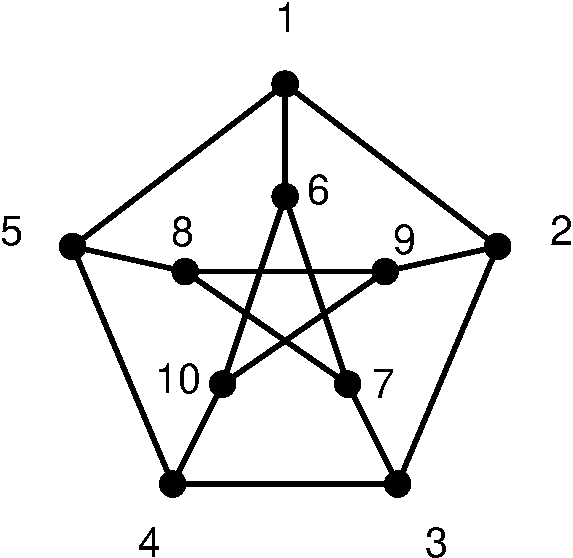
\includegraphics[width=1.5in,clip]{figures/S09_PS5_G1.pdf}}
        \hspace{17mm}
        \subfigure[$G_2$]{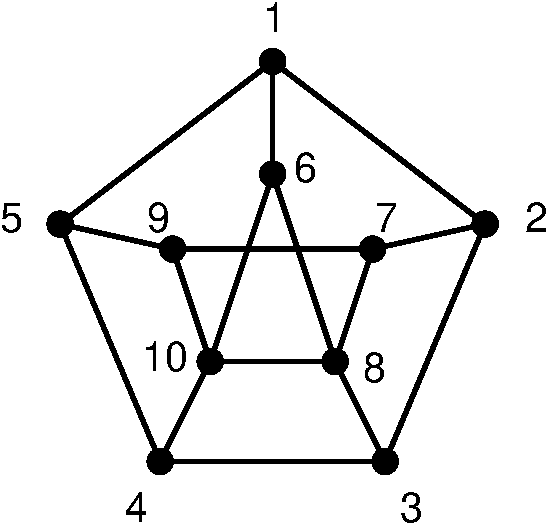
\includegraphics[width=1.5in,clip]{figures/S09_PS5_G4.pdf}} }
\mbox{  \subfigure[$G_3$]{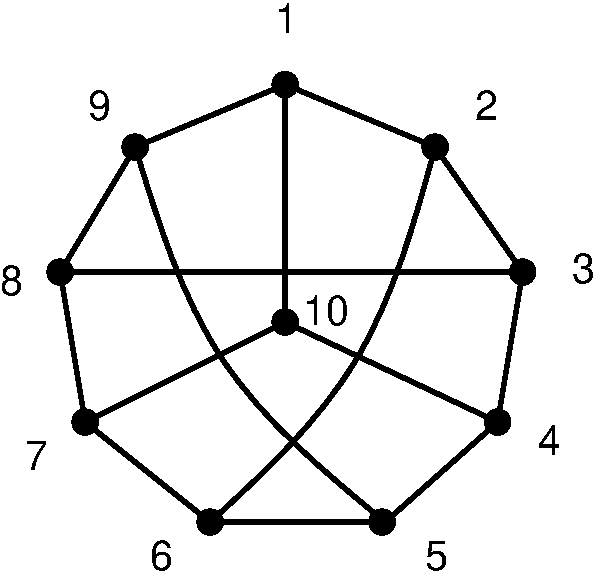
\includegraphics[width=1.5in,clip]{figures/S09_PS5_G2.pdf}}
        \hspace{17mm}
        \subfigure[$G_4$]{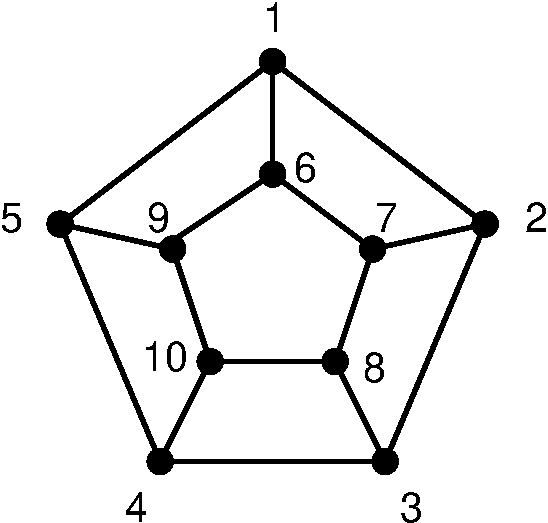
\includegraphics[width=1.5in,clip]{figures/S09_PS5_G3.pdf}}
        }
\end{center}
\caption{Which graphs are isomorphic?}
\label{fig:isog}
\end{figure}


\begin{figure}[h] %[htbp]
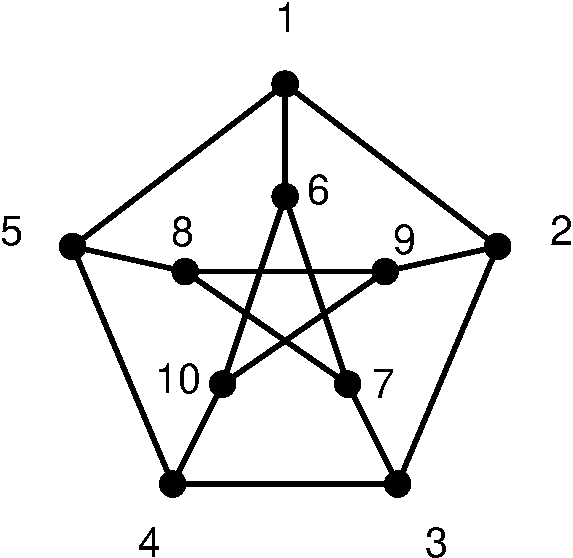
\includegraphics[width=1.5in,clip]{figures/S09_PS5_G1.pdf}
\caption{$G_1$}
\label{fig:G1}
\end{figure}


\begin{figure}[h] %[htbp]
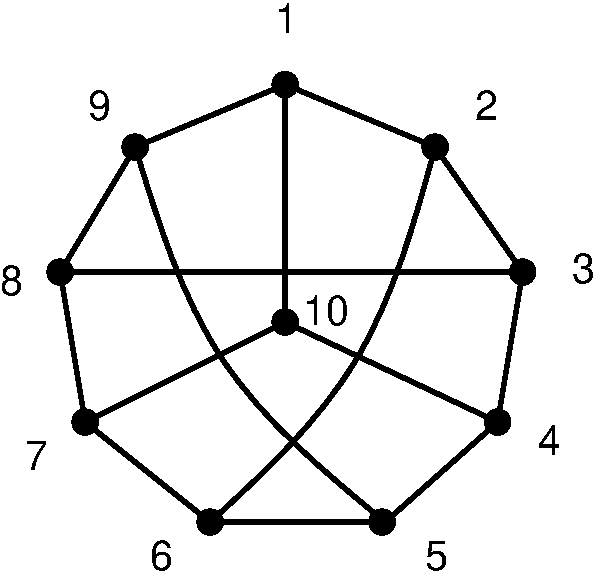
\includegraphics[width=1.5in,clip]{figures/S09_PS5_G2.pdf}
\caption{$G_2$}
\label{fig:G2}
\end{figure}


\begin{figure}[h] %[htbp]
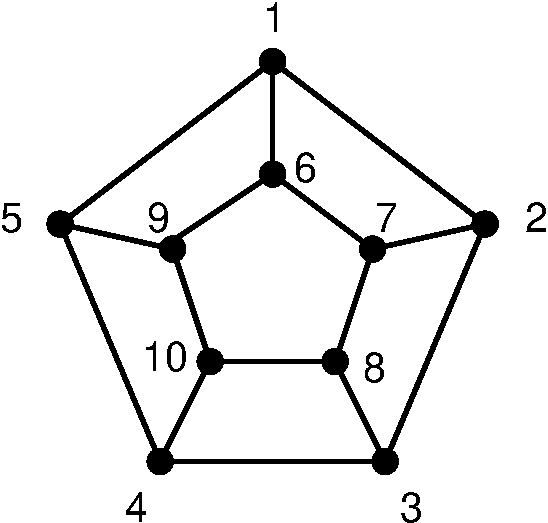
\includegraphics[width=1.5in,clip]{figures/S09_PS5_G3.pdf}
\caption{$G_3$}
\label{fig:G3}
\end{figure}

\begin{figure}[h] %[htbp]
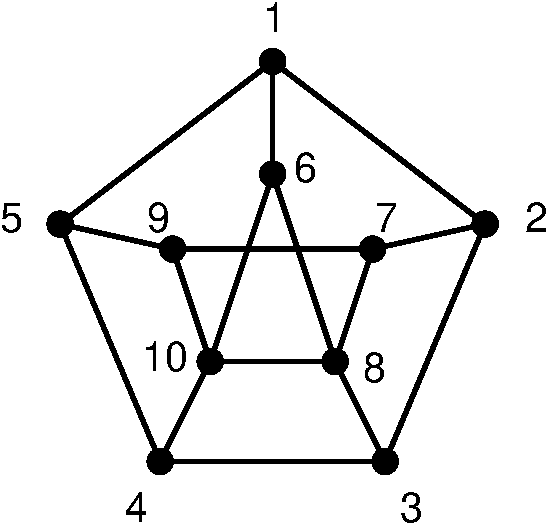
\includegraphics[width=1.5in,clip]{figures/S09_PS5_G4.pdf}
\caption{$G_4$}
\label{fig:G4}
\end{figure}

\begin{solution}
$G_1$ and $G_3$ are isomorphic.  In particular, the function
$f:V_1 \to V_3$ is an isomomorphism, where
\begin{align*}
&f(1)=1 \quad&& f(2)=2 \quad&& f(3)=3 \quad&& f(4)=8 \quad&& f(5)=9 \\
&f(6)=10 \quad&& f(7)=4 \quad&& f(8)=5 \quad&& f(9)=6 \quad&& f(10)=7
\end{align*}

$G_1$ and $G_4$ are not isomorphic to $G_2$: $G_2$ has a vertex of degree
four and neither $G_1$ nor $G_4$ has one.

$G_1$ and $G_4$ are not isomorphic: $G_4$ has a simple cycle of length
four and $G_1$ does not.
\end{solution}

\end{problem}

%%%%%%%%%%%%%%%%%%%%%%%%%%%%%%%%%%%%%%%%%%%%%%%%%%%%%%%%%%%%%%%%%%%%%
% Problem ends here
%%%%%%%%%%%%%%%%%%%%%%%%%%%%%%%%%%%%%%%%%%%%%%%%%%%%%%%%%%%%%%%%%%%%%